\documentclass[a4paper,12pt]{journal}
\usepackage[dvipsnames, svgnames, x11names]{xcolor} 
\usepackage{amsmath}
\usepackage{amssymb}
\usepackage[margin=2.5cm]{geometry}
\usepackage{graphics}
\usepackage{ulem}
\usepackage{setspace}
\usepackage{listings}
\usepackage{algorithm}  
\usepackage{algpseudocode}  
\usepackage{amsmath}  
\usepackage{xcolor}
\usepackage[greek,english]{babel}
\usepackage{chemformula}
\usepackage{wrapfig}
\usepackage{multirow}
\usepackage{booktabs}
\usepackage{fancyhdr}
\usepackage{pgfplots}
\usepackage{tikz}
\usetikzlibrary{positioning} %为了实现相对位置的设定
\pagestyle{fancy}
\usetikzlibrary{math}
\rmfamily
\fancyhf{}
\fancyfoot[R]{\thepage}
\fancyhead[R]{VG441 Midterm}
\title{VG441 Midterm}
\author{Anna Li \\Student ID: 518370910048}
\date{\today}
\lstset{
	columns=fixed,     
	numbers=left,                                        % 在左侧显示行号
	numberstyle=\tiny\color{gray},                       % 设定行号格式
	frame=none,                                          % 不显示背景边框
	backgroundcolor=\color[RGB]{245,245,244},            % 设定背景颜色
	keywordstyle=\color[RGB]{40,40,255},                 % 设定关键字颜色
	numberstyle=\footnotesize\color{darkgray},           
	commentstyle=\it\color[RGB]{0,96,96},                % 设置代码注释的格式
	stringstyle=\ttfamily\slshape\color[RGB]{128,0,0},   % 设置字符串格式
	showstringspaces=false,                              % 不显示字符串中的空格                                        % 设置语言
}
\begin{document}
	\maketitle
	\section*{Problem 1(Forecasting)}
	\subsection*{(a) Scatter plot the demands against time (Figure 1).}
	\begin{figure}[htbp]
		\centering
		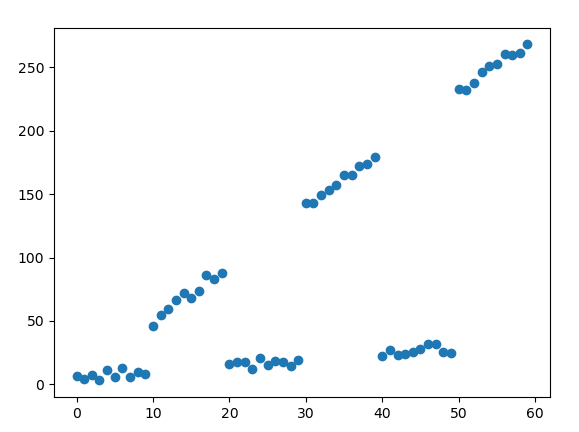
\includegraphics[scale=0.7]{1_a_1.png}
		\caption{demands of time}
	\end{figure}
    Figure 1 is the demands against time
    \subsection*{(b) Run a simple regression and plot your results on top of scatter plot (Figure 2).}
    First, judging from the plot we got, we should use ARIMA model to forecast the data and get:
    \begin{figure}[htbp]
    	\centering
    	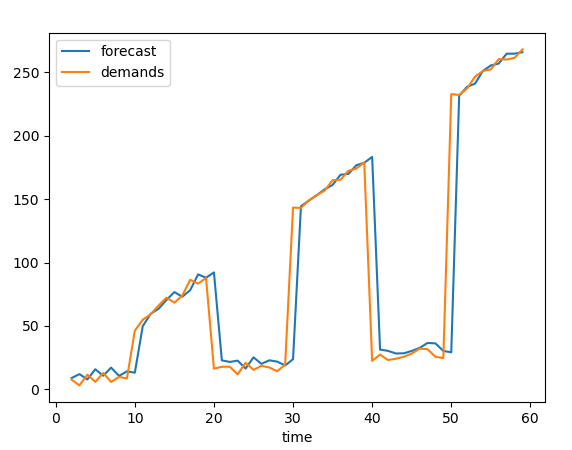
\includegraphics[scale=0.8]{1_b_1.png}
    	\caption{ARIMA model of demands}
    \end{figure}
	\subsection*{(c) Run gradient boosting method with different number of trees:}
	\subsubsection*{1. params = {'n\_estimators': 1, 'max\_depth': 1, 'learning\_rate': 1, 'loss': 'ls'}}
	\begin{figure}[htbp]
		\centering
		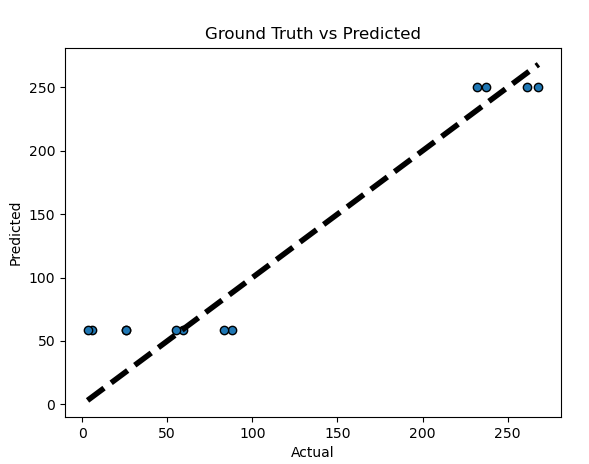
\includegraphics[scale=0.8]{1_c_1.png}
		\caption{results of param:1,1,1,'ls'}
	\end{figure}
	Just as Fig.4 shows, and R2 sq:  0.6959704096715094
	\subsubsection*{2. params = {'n\_estimators': 2, 'max\_depth': 1, 'learning\_rate': 1, 'loss': 'ls'}}
	\begin{figure}[htbp]
		\centering
		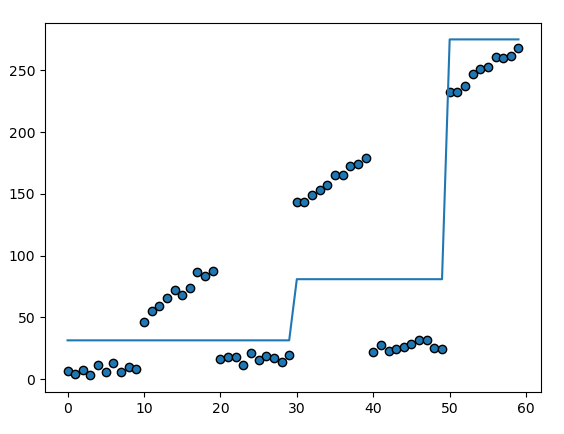
\includegraphics[scale=0.8]{1_c_2.png}
		\caption{results of param:2,1,1,'ls'}
	\end{figure}
	Just as Fig.4 shows, and R2 sq:  0.7290384207566345
	\subsubsection*{3. params = {'n\_estimators': 5, 'max\_depth': 1, 'learning\_rate': 1, 'loss': 'ls'}}
	\begin{figure}[htbp]
		\centering
		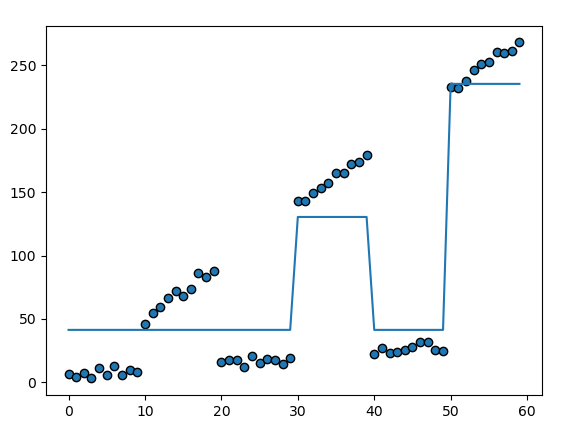
\includegraphics[scale=0.8]{1_c_3.png}
		\caption{results of param:5,1,1,'ls'}
	\end{figure}
	Just as Fig.5 shows, and R2 sq:  0.8860240765658012
	\subsubsection*{4. params = {'n\_estimators': 10, 'max\_depth': 1, 'learning\_rate': 1, 'loss': 'ls'}}
	\begin{figure}[htbp]
		\centering
		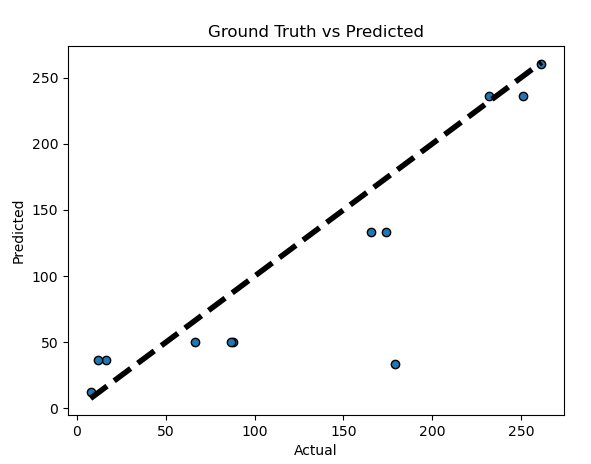
\includegraphics[scale=0.8]{1_c_4.png}
		\caption{results of param:10,1,1,'ls'}
	\end{figure}
	Just as Fig.6 shows, and R2 sq:  0.9751642096479143
	\subsubsection*{5. params = {'n\_estimators': 20, 'max\_depth': 1, 'learning\_rate': 1, 'loss': 'ls'}}
	\begin{figure}[htbp]
		\centering
		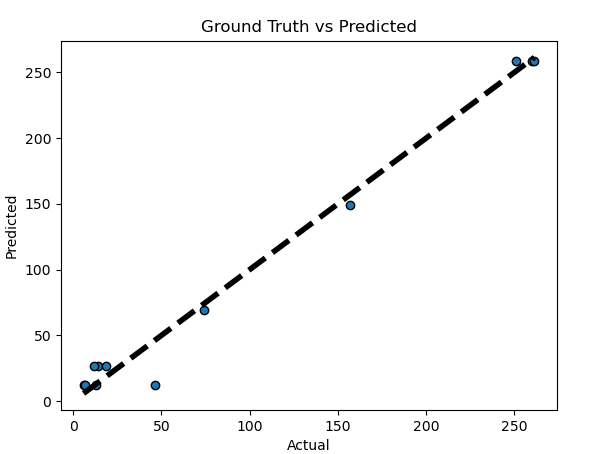
\includegraphics[scale=0.8]{1_c_5.png}
		\caption{results of param:20,1,1,'ls'}
	\end{figure}
	Just as Fig.7 shows, and R2 sq:  0.9875429979290639
	\subsubsection*{5. params = {'n\_estimators': 50, 'max\_depth': 1, 'learning\_rate': 1, 'loss': 'ls'}}
	\begin{figure}[htbp]
		\centering
		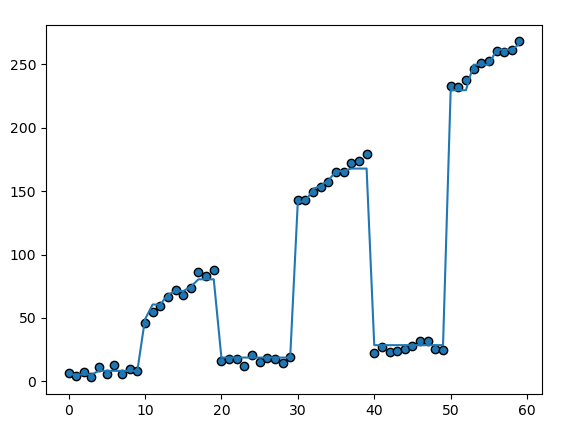
\includegraphics[scale=0.8]{1_c_6.png}
		\caption{results of param:50,1,1,'ls'}
	\end{figure}
	Just as Fig.8 shows, and R2 sq:  0.9981772426017594
	\section*{Problem 2 (Quantity-Discount Model)}
	\subsection*{(a) What is the optimal ordering strategy?}
	From the question, 
	\begin{equation}
		K=50\text{\$ /order}\quad h=200/12\text{\$ /(unit* month)}\quad \lambda=50\text{units/month}\quad c=\left\{\begin{array}{l l}
				520&, x<12\\
				510&, 12\leq x\leq 64\\
				495&, 65\leq x\leq 128\\
				485&, x>128\\
		\end{array}\right.
	\end{equation}
	Therefore, we use the All-unit Discount:
	For this structure, we could generate the $g(Q)$, and get that:
	\begin{equation}
		\begin{array}{r c l}
			g_0(Q)&=&520*50+50*50/Q+200/12*520/2*Q\\
			g_1(Q)&=&510*50+50*50/Q+200/12*510/2*Q\\
			g_2(Q)&=&495*50+50*50/Q+200/12*495/2*Q\\
			g_3(Q)&=&485*50+50*50/Q+200/12*485/2*Q\\
		\end{array}
	\end{equation}
	And we could draw the graph like:
	\begin{figure}[h]
		\begin{tikzpicture}
			
			\begin{axis}[
				axis x line=middle,
				axis y line=middle,
				ylabel=$g(Q)$,
				xlabel=$Q$
				]
				\addplot[domain=0:12]{26000+2500/x+4333.33*x};
				\addplot[domain=12:64]{25500+2500/x+4250*x};
				\addplot[domain=65:128]{24750+2500/x+4125*x};
				\addplot[domain=128:200]{24250+2500/x+4041.67*x};
			\end{axis}
		\end{tikzpicture}
		\caption{Total cost for all-units quantity discount structure}
	\end{figure}
	and the $Q_j^\ast$ is:
	\begin{equation}
		\begin{array}{r c l}
			Q_0^\ast&=&0.76\\
			Q_1^\ast&=&0.77\\
			Q_2^\ast&=&0.78\\
			Q_3^\ast&=&0.79\\
		\end{array}
	\end{equation}
	Among these value, $Q_0^\ast$ is feasible, which is:
	$$g_0(1)=32833.3$$
	Then we caculare the cost of breakpoints to the right of $Q_1^\ast$and get:\\
	$$g_0(12)=78208.3$$
	Therefore, the optimal orfer quantity is $Q=1$, which incurs a total monthly cost of 32833.3\$
	\subsection*{(b)The supplier has offered to be a drop shipper, i.e., they will ship directly to the customer. In exchange, they will increase the unit price to \$520 per computer, but not charge the ordering costs and all inventory will be held at the supplier. From a purely financial standpoint, should Zeus take them up on the offer?}
	According to the question, we could get this results:
	\begin{equation}
			\lambda=50\text{units/month}\quad c=520\$/unit
	\end{equation}
	Therefore, we can list the equation that 
	\begin{equation}
		\text{Average Cycle cost}=26000\$/month
	\end{equation}
	Therefore, Zeus should take them up on the offer.
	\section*{Problem 3 (Wagner-Whitin Model)}
	\subsection*{(a) Use dynamic programming to solve the problem (on paper by hands).}
	First, we read from question and get the equation that:\\
	\begin{equation}
		K=1000\quad h=1.2
	\end{equation}
	Then we apply the dynamic programming and get:\\
	\begin{equation}
		\begin{aligned}
			\theta_8&=0\\
			\theta_7&=1000+1.2(0\cdot d_7)+\theta_8\\
			&=1000\text{[s(7)=8]}\\
			\theta_6&=\min\{1000+1.2(0\cdot d_6)+\theta_7,1000+1.2(0\cdot d_6+1\cdot d_7)+\theta_8\}\\
			&=\min\{2000,1348\}\\
			&=1348\text{[s(6)=8]}\\
			\theta_5&=\min\{1000+1.2(0\cdot d_5)+\theta_6,1000+1.2(0\cdot d_5+1\cdot d_6)+\theta_7,\\
			&1000+1.2(0\cdot d_5+1\cdot d_6+2\cdot d_7)+\theta_8\}\\
			&=\min\{2348,2252,1948\}\\
			&=1948\text{[s(5)=8]}\\
			\theta_4&=\min\{1000+1.2(0\cdot d_4)+\theta_5,1000+1.2(0\cdot d_4+1\cdot d_5)+\theta_6,\\
			&1000+1.2(0\cdot d_4+1\cdot d_5+2\cdot d_6)+\theta_7,\\
			& 1000+1.2(0\cdot d_4+1\cdot d_5+2\cdot d_6+3
		\cdot d_7)+\theta_8\}\\
			&=\min\{2948,2552,2708,2752\}\\
			&=2552\text{[s(4)=6]}\\
			\theta_3&=\min\{1000+1.2(0\cdot d_3)+\theta_4,1000+1.2(0\cdot d_3+1\cdot d_4)+\theta_5,\\
			&1000+1.2(0\cdot d_3+1\cdot d_4+2\cdot d_5)+\theta_6,\\
			& 1000+1.2(0\cdot d_3+1\cdot d_4+2\cdot d_5+3
			\cdot d_6)+\theta_7,\\
			&1000+1.2(0\cdot d_3+1\cdot d_4+2\cdot d_5+3
			\cdot d_6+4\cdot d_7)+\theta_8\}\\
			&=\min\{3552,3056,2864,3272,3664\}\\
			&=2864\text{[s(3)=6]}\\
			\theta_2&=\min\{1000+1.2(0\cdot d_2)+\theta_3,1000+1.2(0\cdot d_2+1\cdot d_3)+\theta_4,\\
			&1000+1.2(0\cdot d_2+1\cdot d_3+2\cdot d_4)+\theta_5,\\
			& 1000+1.2(0\cdot d_2+1\cdot d_3+2\cdot d_4+3
			\cdot d_5)+\theta_6,\\
			&1000+1.2(0\cdot d_2+1\cdot d_3+2\cdot d_4+3
			\cdot d_5+4\cdot d_6)+\theta_7,\\
			&1000+1.2(0\cdot d_2+1\cdot d_3+2\cdot d_4+3
			\cdot d_5+4\cdot d_6+5\cdot d_7)+\theta_8\}\\
			&=\min\{3864,3678,3290,3302,3962,4702\}\\
			&=3290\text{[s(2)=5]}\\
			\theta_1&=\min\{1000+1.2(0\cdot d_1)+\theta_2,1000+1.2(0\cdot d_1+1\cdot d_2)+\theta_3,\\
			&1000+1.2(0\cdot d_1+1\cdot d_2+2\cdot d_3)+\theta_4,\\
			& 1000+1.2(0\cdot d_1+1\cdot d_2+2\cdot d_3+3
			\cdot d_4)+\theta_5,\\
			&1000+1.2(0\cdot d_1+1\cdot d_2+2\cdot d_3+3
			\cdot d_4+4\cdot d_5)+\theta_6,\\
			&1000+1.2(0\cdot d_1+1\cdot d_2+2\cdot d_3+3
			\cdot d_4+4\cdot d_5+5\cdot d_6)+\theta_7,\\
			&1000+1.2(0\cdot d_1+1\cdot d_2+2\cdot d_3+3
			\cdot d_4+4\cdot d_5+5\cdot d_6+6\cdot d_7)+\theta_8\}\\
			&=\{4290,4050,3990,3710,3926,4838,5926\}\\
			&=3710\text{s(1)=5}
		\end{aligned}
	\end{equation}
Therefore, we could get that the best choice is:\\
Order 570 on Sunday, order 670 on Thursday
	\subsection*{(b) Formulate as a shortest path problem and draw the corresponding diagram with nodes, edges, and edge costs. Solve using Dijkstra’s algorithm (on paper by hands).}
	
\begin{tikzpicture}[
		roundnode/.style={circle,draw=black!60, fill=gray!5, very thick, minimum size=7mm},
		]
		\node[roundnode] (Sunday) {1};
		\node[roundnode] (Monday) [right=of Sunday]{2};
		\node[roundnode] (Tuesday) [right=of Monday]{3};
		\node[roundnode] (Wednesday) [right=of Tuesday]{4};
		\node[roundnode] (Thursday)[right=of Wednesday] {5};
		\node[roundnode] (Friday) [right=of Thursday]{6};
		\node[roundnode] (Saturday) [right=of Friday]{7};
		\node[roundnode] (Finalday) [right=of Saturday]{8};
		
	\end{tikzpicture}\\
	And by applying the Dikstra's algorithm, we could conclude that:
	\begin{center}
		\begin{tabular}{c c c c}
			Number of steps&X&A[s]&B[s]\\
			1&2,3,4,5,6,7,8&0&$\emptyset$\\
			2&3,4,5,6,7,8&A[2]=1000&B[2]=\{1-2\}\\
			3&4,5,6,7,8&A[3]=1186&B[4]=\{1-3\}\\
			4&5,6,7,8&A[4]=1438&B[4]=\{1-4\}\\
			5&6,7,8&A[5]=1762&B[5]=\{1-5\}\\
			6&7,8&A[6]=2578&B[6]=\{1-6\}\\
			7&8&A[7]=3014&B[7]=\{1-5-7\}\\
			8&$\emptyset$&A[8]=3710&B[8]=\{1-5-8\}\\
		\end{tabular}
	\end{center}
	\subsection*{(c) Formulate the problem as a MILP on paper and solve it in Python.}
	We want to minimize: 
	\section*{Problem 4 (Linear Programming Duality)}
	\subsection*{(a) Please write down duality of the following linear programming problem.}
	\begin{equation}
		\begin{aligned}
			min\quad&24y_1+60y_2\\
			s.t.\quad&3y_1+y_2\geq 6\\
			&2y_1+2y_2\leq 14\\
			&y_1+4y_2= 13\\
			&y_1\geq 0\\
			&y_2\leq 0\\
		\end{aligned}
	\end{equation}
	\subsection*{(b) Bipartite graph is a special graph. Its vertices are divided into two separate sets and edges only exist between those two sets.}
	suppose we have n nodes in I and m nodes in J, 
	\begin{equation}
		\begin{aligned}
			min\quad &\sum_{i:(i,j)\in E}y_i+\sum_{j:(i,j)\in E}y_{n+j}\\
			s.t.\quad &
		\end{aligned}
	\end{equation}
\end{document}
